\documentclass{article}
\usepackage[T1,T2A]{fontenc}
\usepackage[utf8]{inputenc}
\usepackage[english,ukrainian]{babel}
\usepackage[]{amsthm} %lets us use \begin{proof}
\usepackage[]{amssymb} %gives us the character \varnothing
\usepackage{amsmath}
\usepackage{graphicx}

\begin{document}

\title{Домашка 5. Графи, дерева}
\date{22 червня 2023}

\maketitle

\subsection*{Задача 1}
Наступні графи задані матрицею суміжності. Аналізуючи матрицю скажіть чи граф зв'язний, двудольний? Знайдіть кількість
ланцюгів довжини 2 і 3 з кожної вершини в кожну.
\begin{itemize}
    \item
        $\begin{bmatrix}
            0,1,0,0 \\
            1,0,0,0 \\
            0,0,1,1 \\
            0,0,1,1
        \end{bmatrix}$
    \item
        $\begin{bmatrix}
            0,0,1,2 \\
            0,0,1,0 \\
            1,1,0,0 \\
            2,0,0,0
        \end{bmatrix}$
    \item
        $\begin{bmatrix}
            1,2,3,1 \\
            2,0,1,1 \\
            3,1,0,2 \\
            1,1,2,0
        \end{bmatrix}$
\end{itemize}

\subsection*{Задача 2}
Скільки існує класів еквівалентості по ізоморфізму серед дерев на 5 вершинах? на 6? Наведіть усі і доведіть.

\subsection*{Задача 3}
Намалюйте граф або доведіть, що його не існує
\begin{itemize}
    \item Дерево, 6 вершин, 5 ребер
    \item Дерево, 8 вершин, 10 ребер
    \item Дерево, 7 вершин, 5 ребер
    \item Дерево, 5 вершин, сума всіх степенів вершин 10
    \item Зв'язний граф, у якому є нетривіальний цикл, 12 вершин, 9 ребер
    \item Зв'язний граф, у якому є нетривіальний цикл, 7 вершин, 8 ребер
\end{itemize}

\subsection*{Задача 4}
Чи ізоморфіні наступні пари графів? Доведіть.

\begin{figure}[h]
\centering
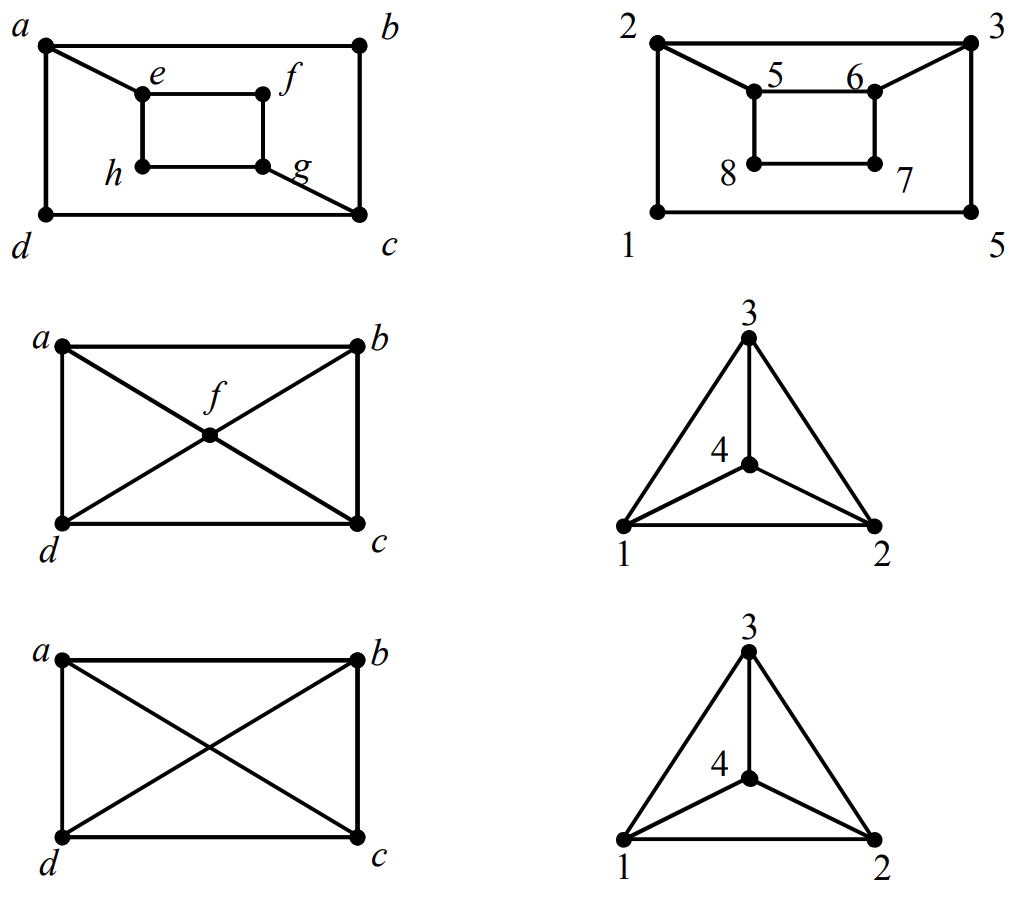
\includegraphics[width=90mm]{h1}
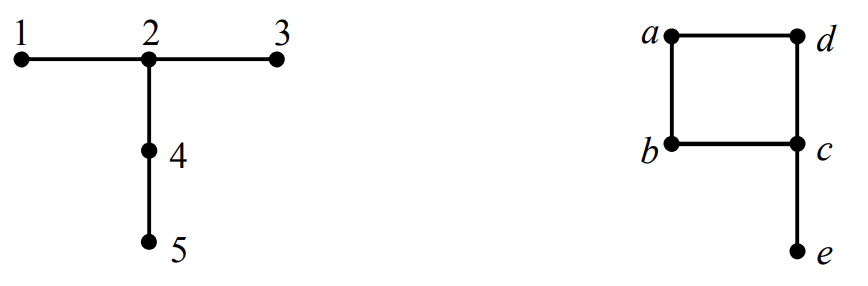
\includegraphics[width=90mm]{h2}
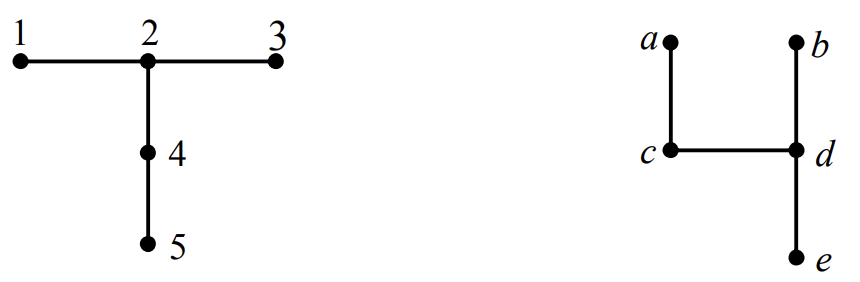
\includegraphics[width=90mm]{h3}
\end{figure}


\end{document}